\subsection{Plate with hole problem}
Consider an infinite plate with a hole centered at the origin, as shown in Figure \ref{fg:plate_with_hole_model}, and at the infinity towards the $x$-direction subjected to a uniform traction $T=1000$. The geometric and material parameters for this problem are that the ratio of the hole $a=1$, Young's modulus $E=3\times 10^6$, and Poisson's ratio $\nu = 0.5-10^{-8}$. The analytical solution of this problem refers to the Michell solution \cite{timoshenko1969} as:
\begin{equation}\label{plate_with_hole_exact}
\left\{
\begin{aligned}
u_x(\rho,\theta)&=\frac{Ta}{8\mu}\left( \frac{\rho}{a}(k+1)\cos\theta - \frac{2a^3}{\rho^3}\cos3\theta + \frac{2a}{\rho}((1+k)\cos\theta + \cos3\theta) \right) \\
u_y(\rho,\theta)&=\frac{Ta}{8\mu}\left( \frac{\rho}{a}(k-3)\sin\theta - \frac{2a^3}{\rho^3}\sin3\theta + \frac{2a}{\rho}((1-k)\sin\theta + \sin3\theta) \right)
\end{aligned}
\right.
\end{equation}
in which $k = \frac{3-\nu}{1+\nu}$, $\mu = \frac{E}{2(1+\nu)}$. And the stress components are given by:
\begin{equation}
\left\{
\begin{aligned}
\sigma_{xx}&=T\left( 1 - \frac{a^2}{\rho^2}\left( \frac{3}{2}\cos2\theta + \cos4\theta \right) + \frac{3a^4}{2\rho^4}\cos4\theta \right) \\
\sigma_{yy}&=-T\left( \frac{a^2}{\rho^2}\left( \frac{1}{2}\cos2\theta - \cos4\theta \right) + \frac{3a^4}{2\rho^4}\cos4\theta \right) \\
\sigma_{xy}&=-T\left( \frac{a^2}{\rho^2}\left( \frac{1}{2}\sin2\theta + \sin4\theta \right) - \frac{3a^4}{2\rho^4}\sin4\theta \right) \\
\end{aligned}
\right.
\end{equation}

According to the symmetry property of this problem, only a quarter model with length $b=5$ is considered as shown in Figure \ref{fg:plate_with_hole_model}. The displacement is discretized by 3-node and 6-node triangular elements with $81$, $299$, $1089$, and $4225$ nodes. The corresponding linear and quadratic meshfree formulations are employed for pressure discretization, and the characterized support sizes are chosen as 1.5 and 2.5, respectively. Figure \ref{fg:plate_with_hole_ns} studies the relationship between strain, pressure errors, and $n_p$. Unlike the quadrilateral element case in Section \ref{sec:cantilever}, the quadratic Tri6--RK shows worse results while the constraint ratio is out of the optimal range. And Tri3--RK exhibits less sensitivity in strain error than Tri6--RK, but its error is increasing while $n_p$ goes up. Both Tri3--RK and Tri6--RK with constraint ratios under the optimal range perform acceptably. The corresponding error convergence study is presented in Figure \ref{fg:plate_with_hole_convergence}, and only Tri3--RK with $r=2$ shows a comparable result with the optimal one with $r=r_{opt}$. The other formulations with the traditional constraint ratio show lower accuracy and error convergence rates.

\begin{figure}[H]
\centering
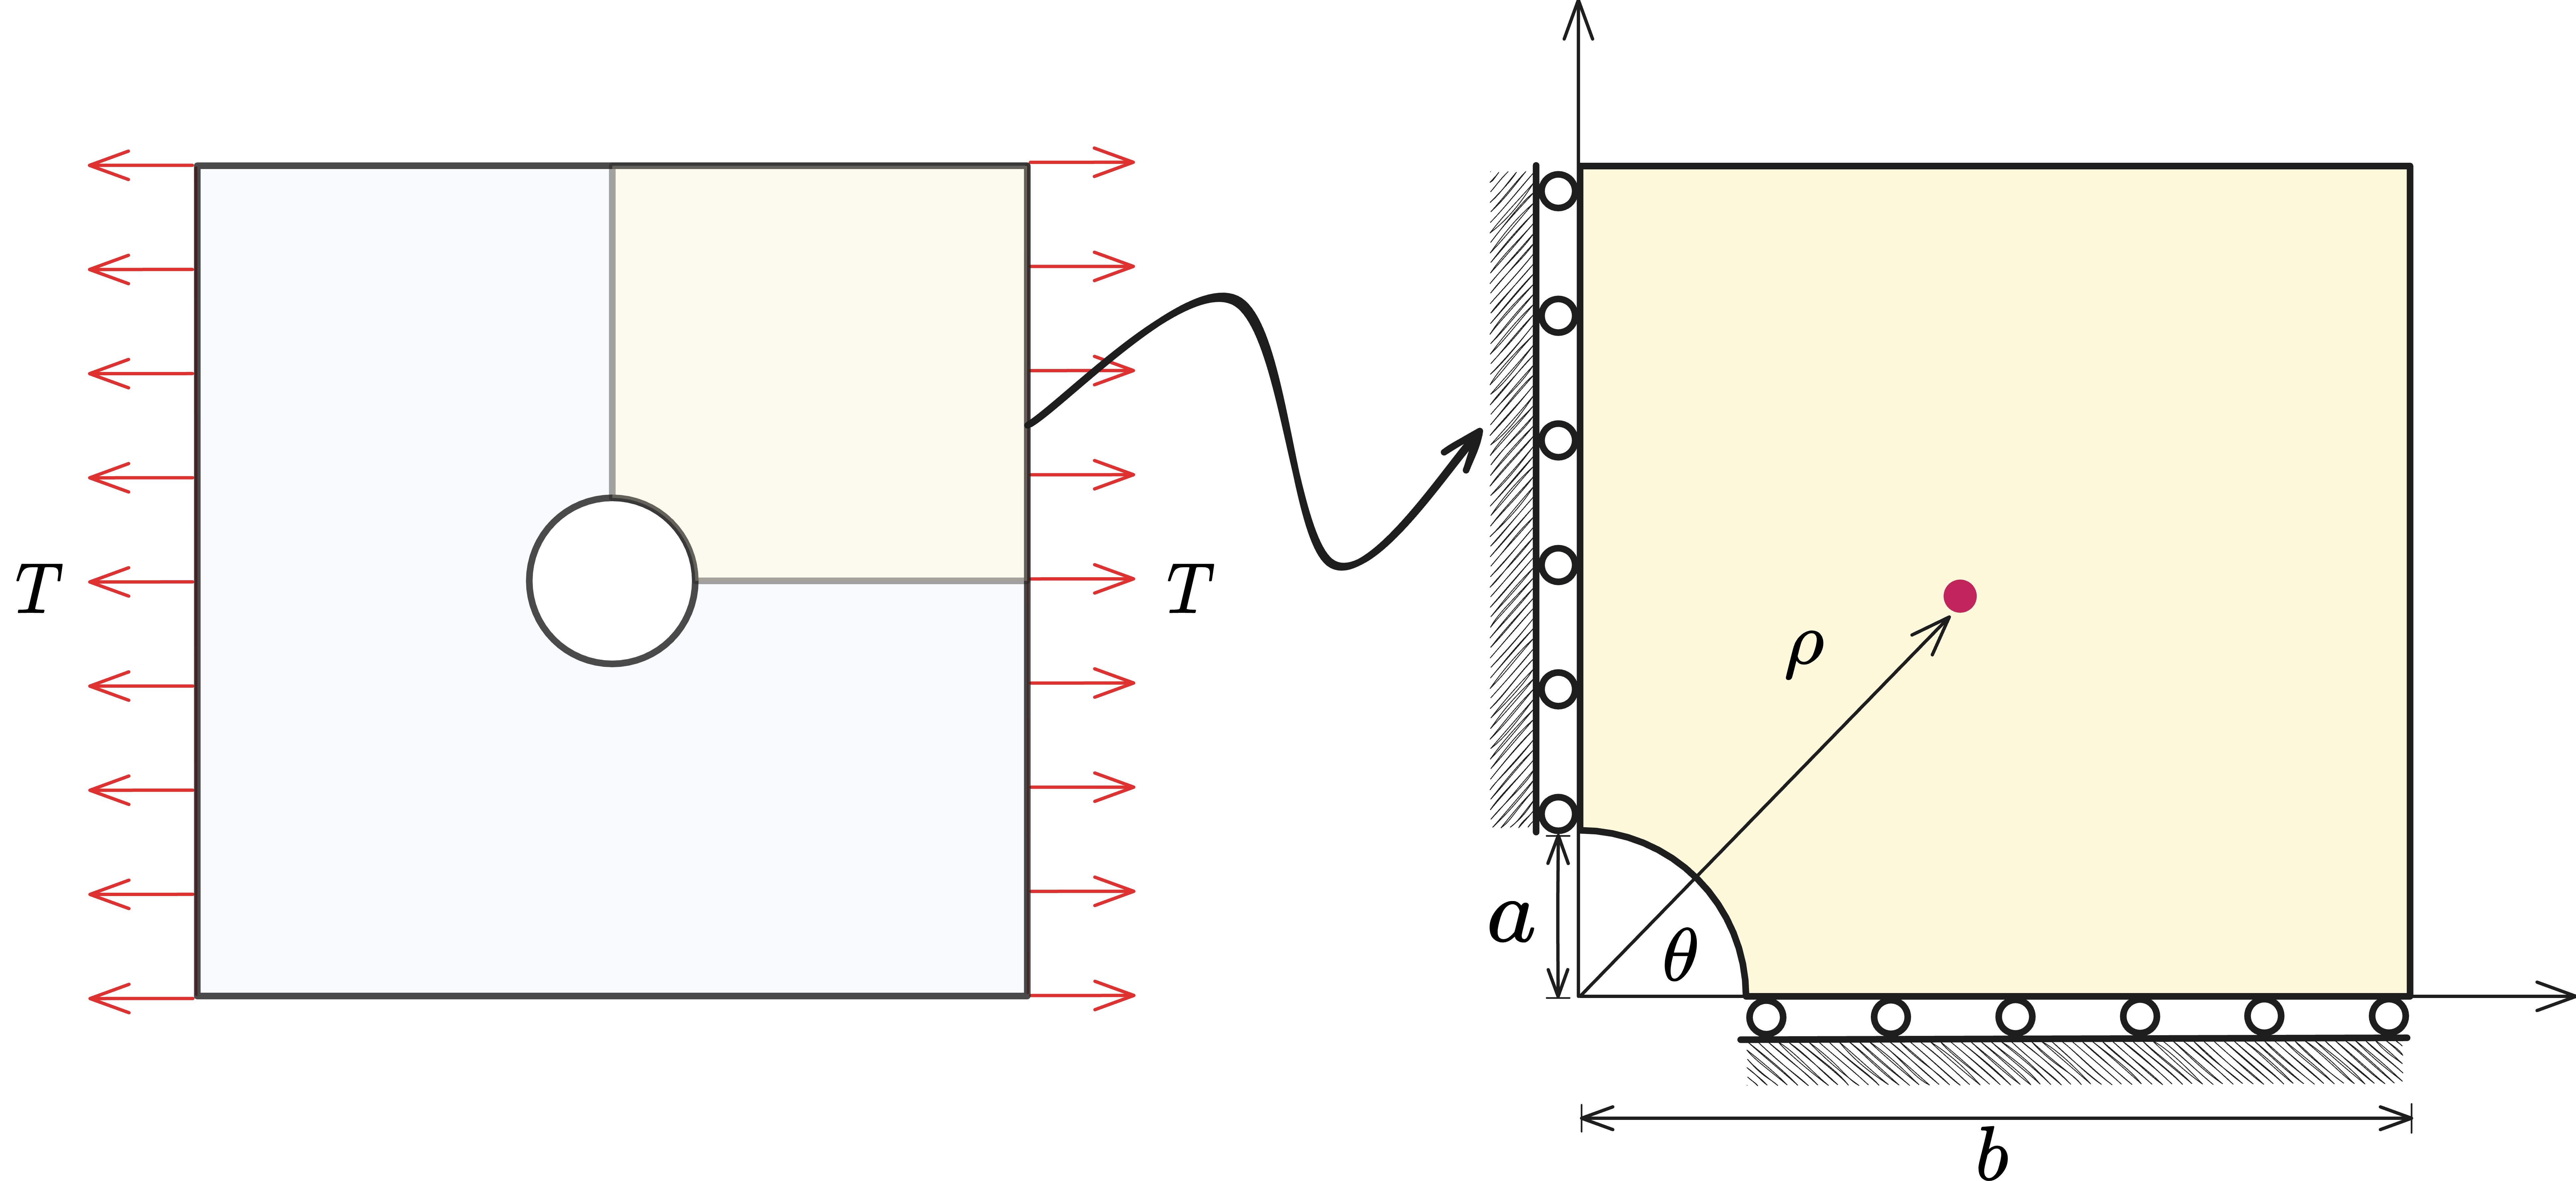
\includegraphics[width=\textwidth]{png/plate_with_hole_model.png}
\caption{Illustration of plate with hole problem}\label{fg:plate_with_hole_model}
\end{figure}

\begin{figure}[H]
\centering
\begin{tabular}{c@{\hspace{0pt}}c}
$\Vert \boldsymbol{u} - \boldsymbol{u}_h \Vert_V$ & $\Vert p - p_h \Vert_Q$ \\
\raisebox{-0.7\height}{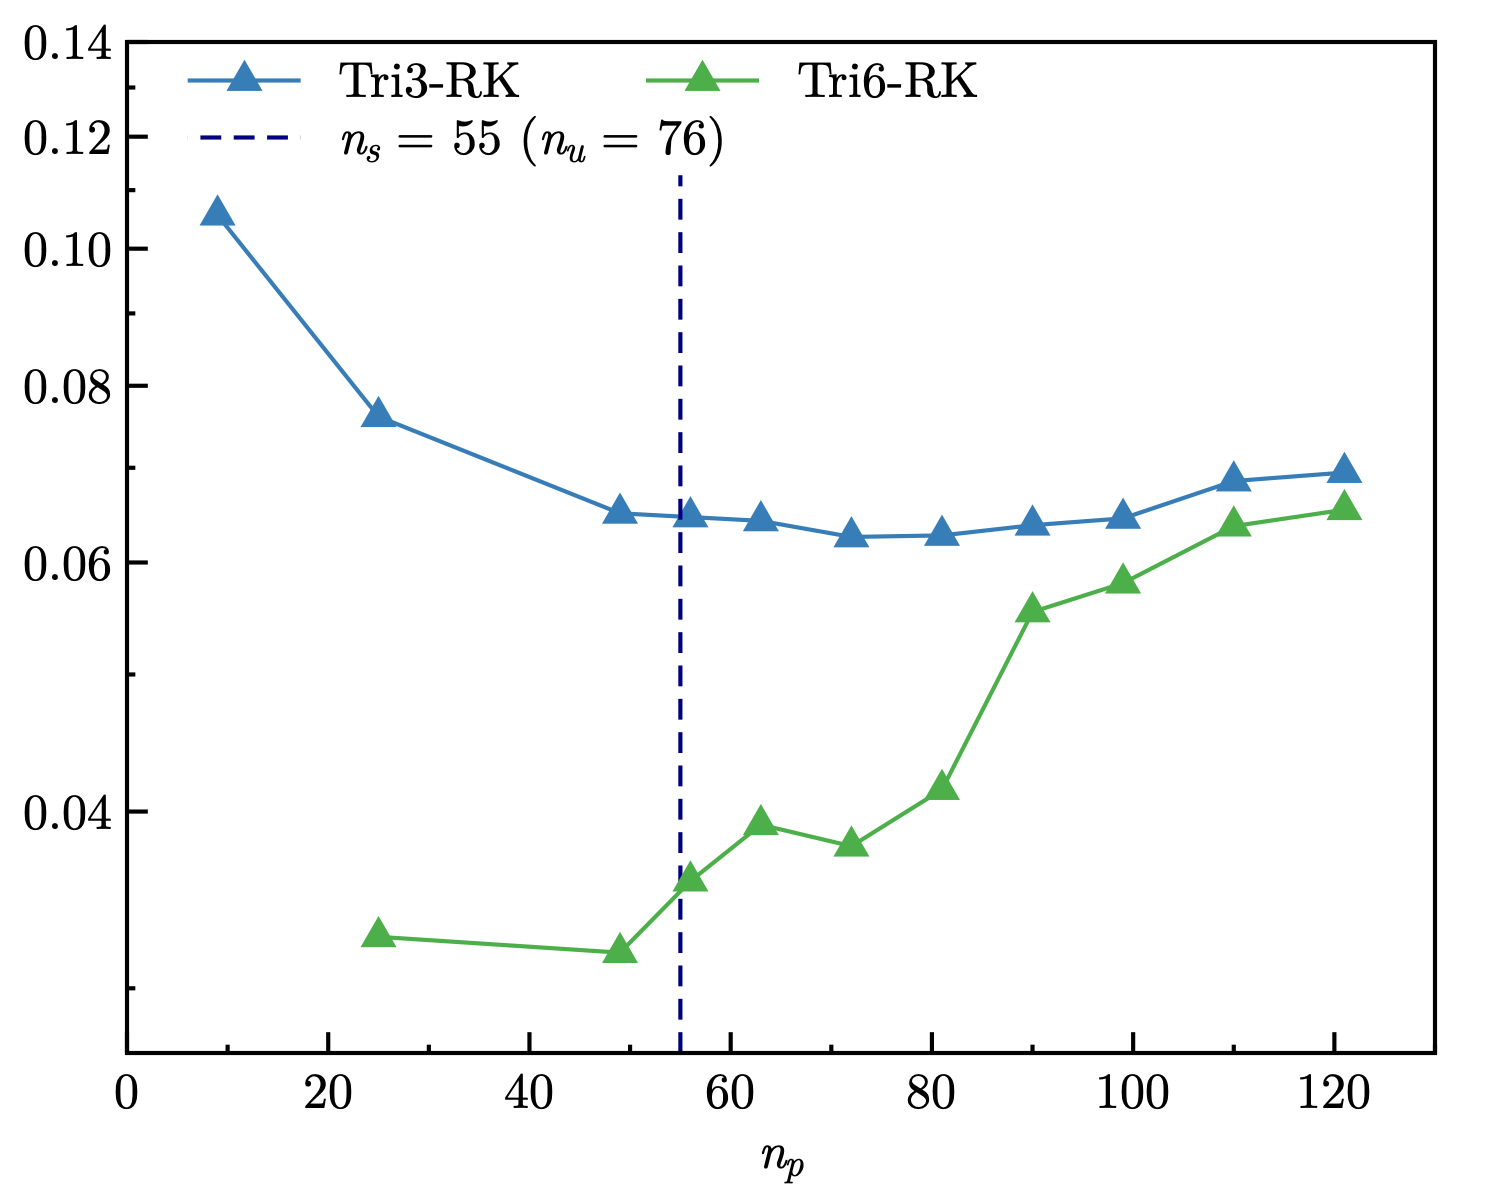
\includegraphics[width=0.48\textwidth]{png/plate_Hdev_4.png}}
& \raisebox{-0.7\height}{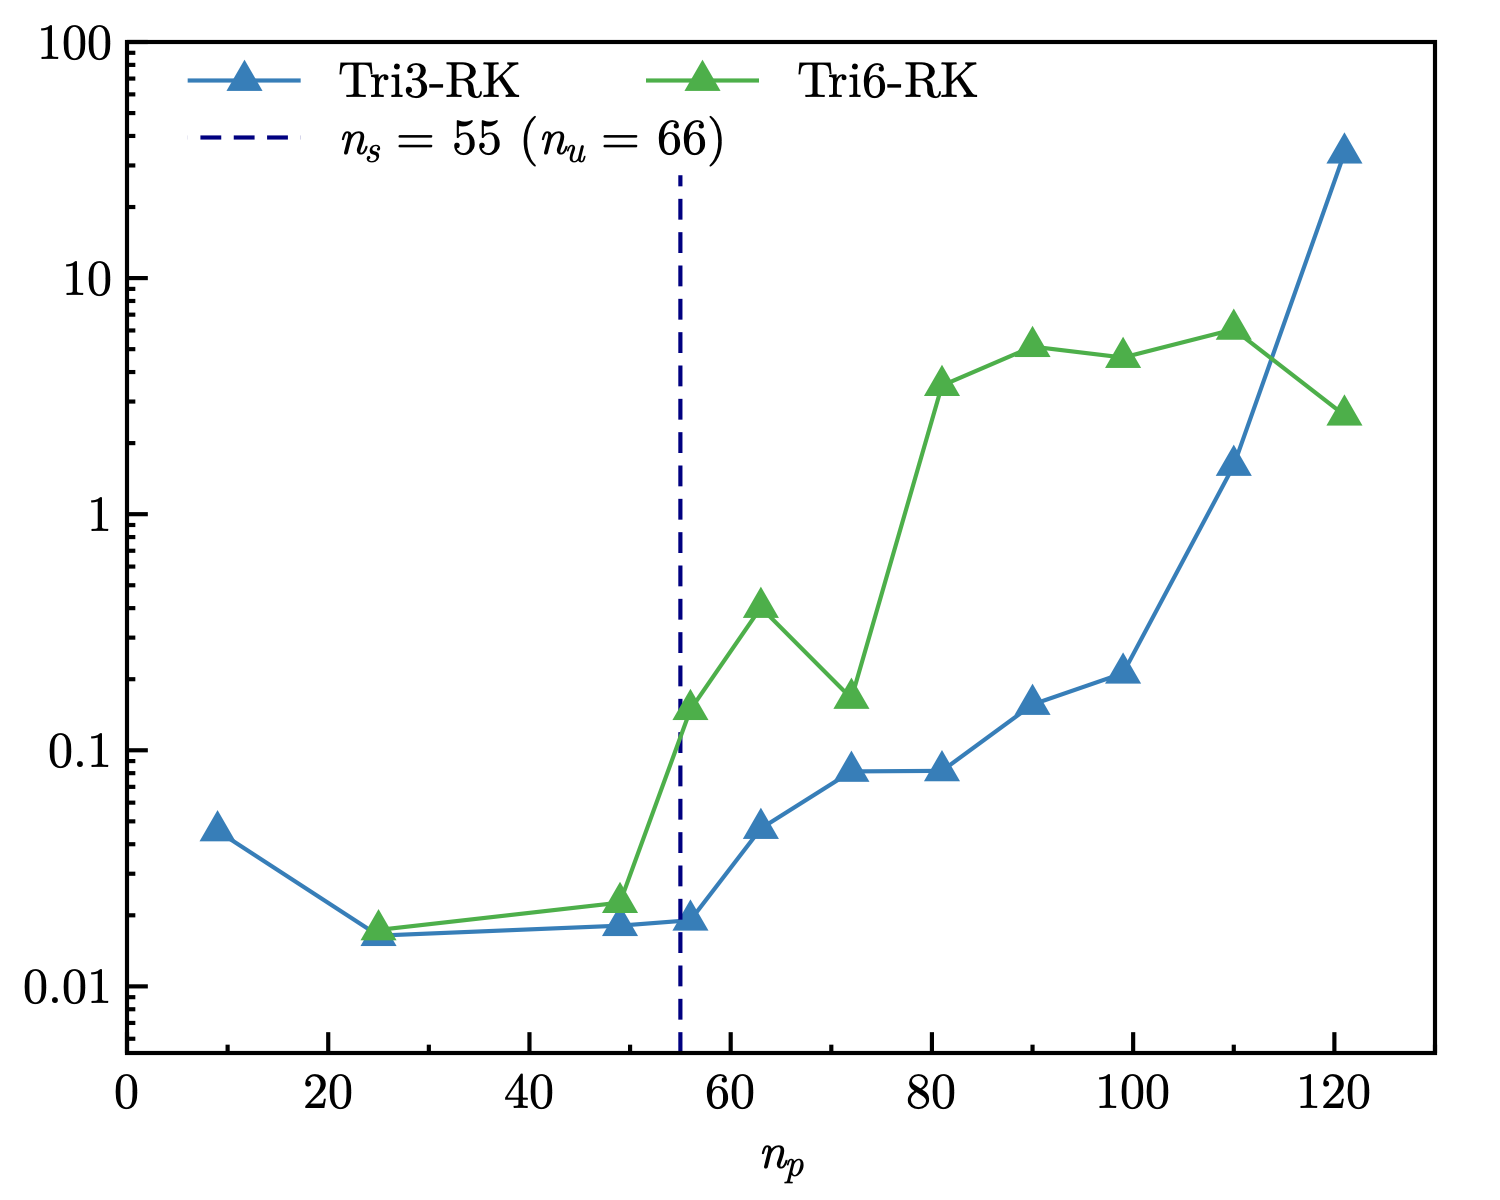
\includegraphics[width=0.48\textwidth]{png/plate_L2_p_4.png}} \\
\raisebox{-0.7\height}{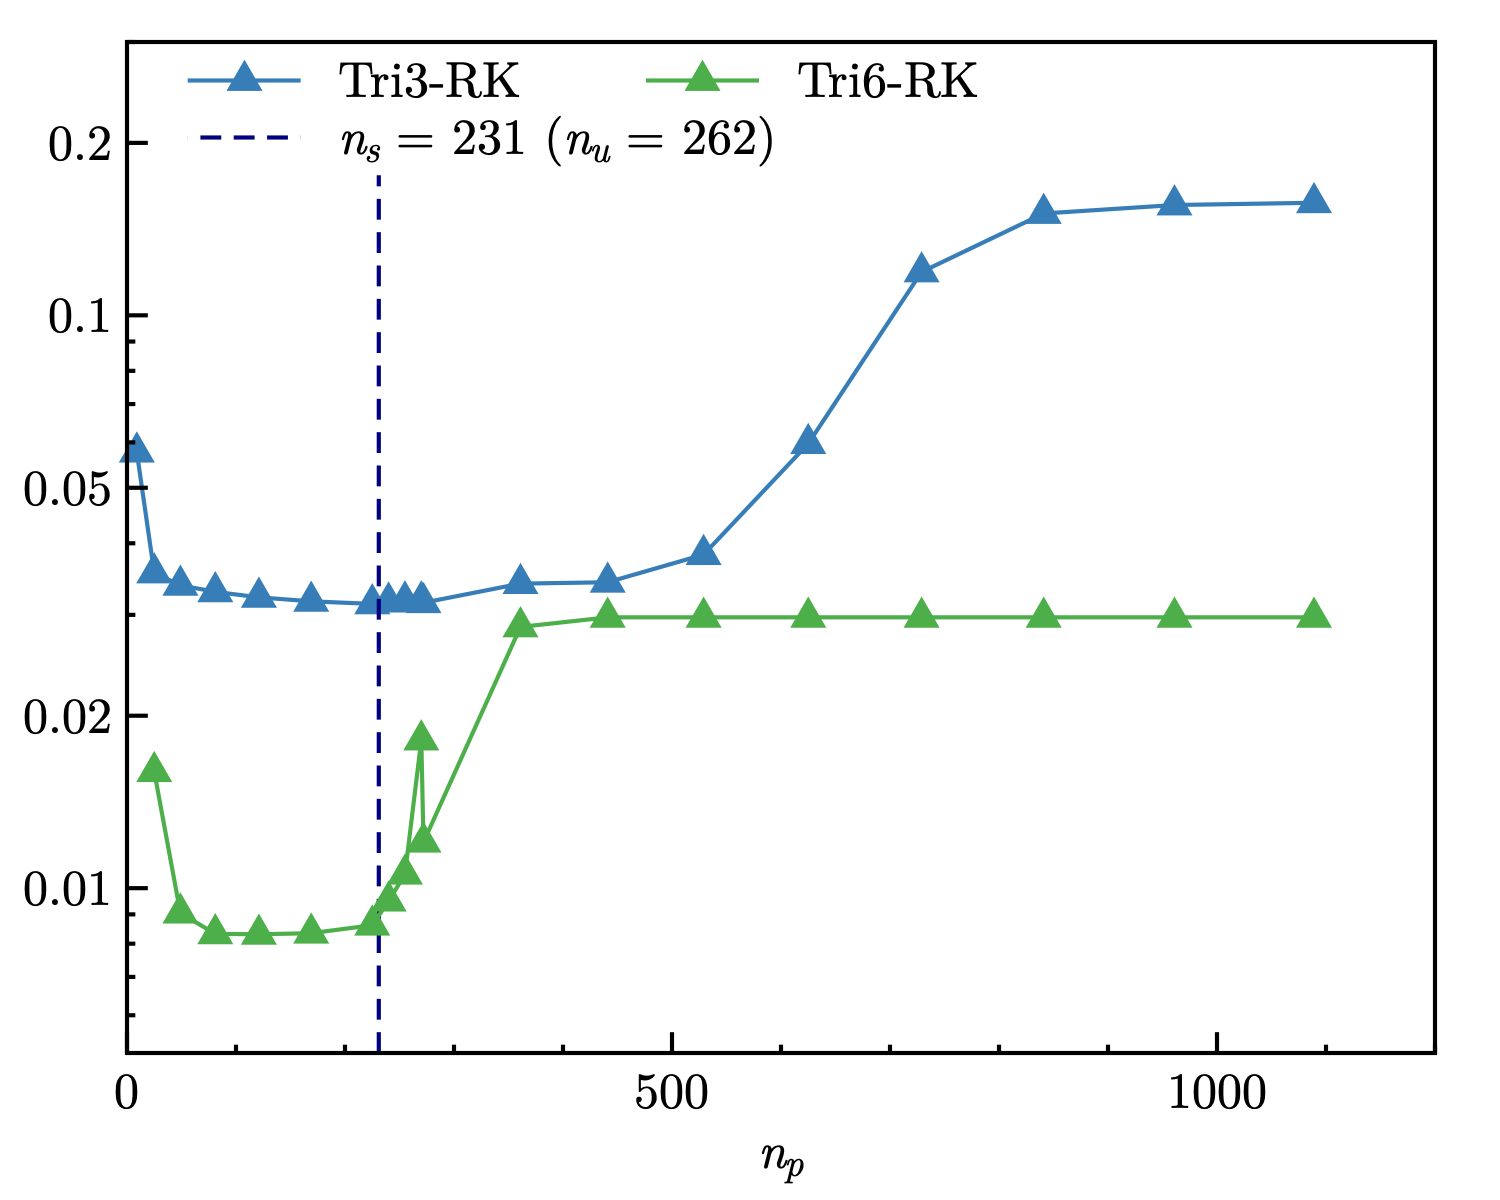
\includegraphics[width=0.48\textwidth]{png/plate_Hdev_8.png}}
& \raisebox{-0.7\height}{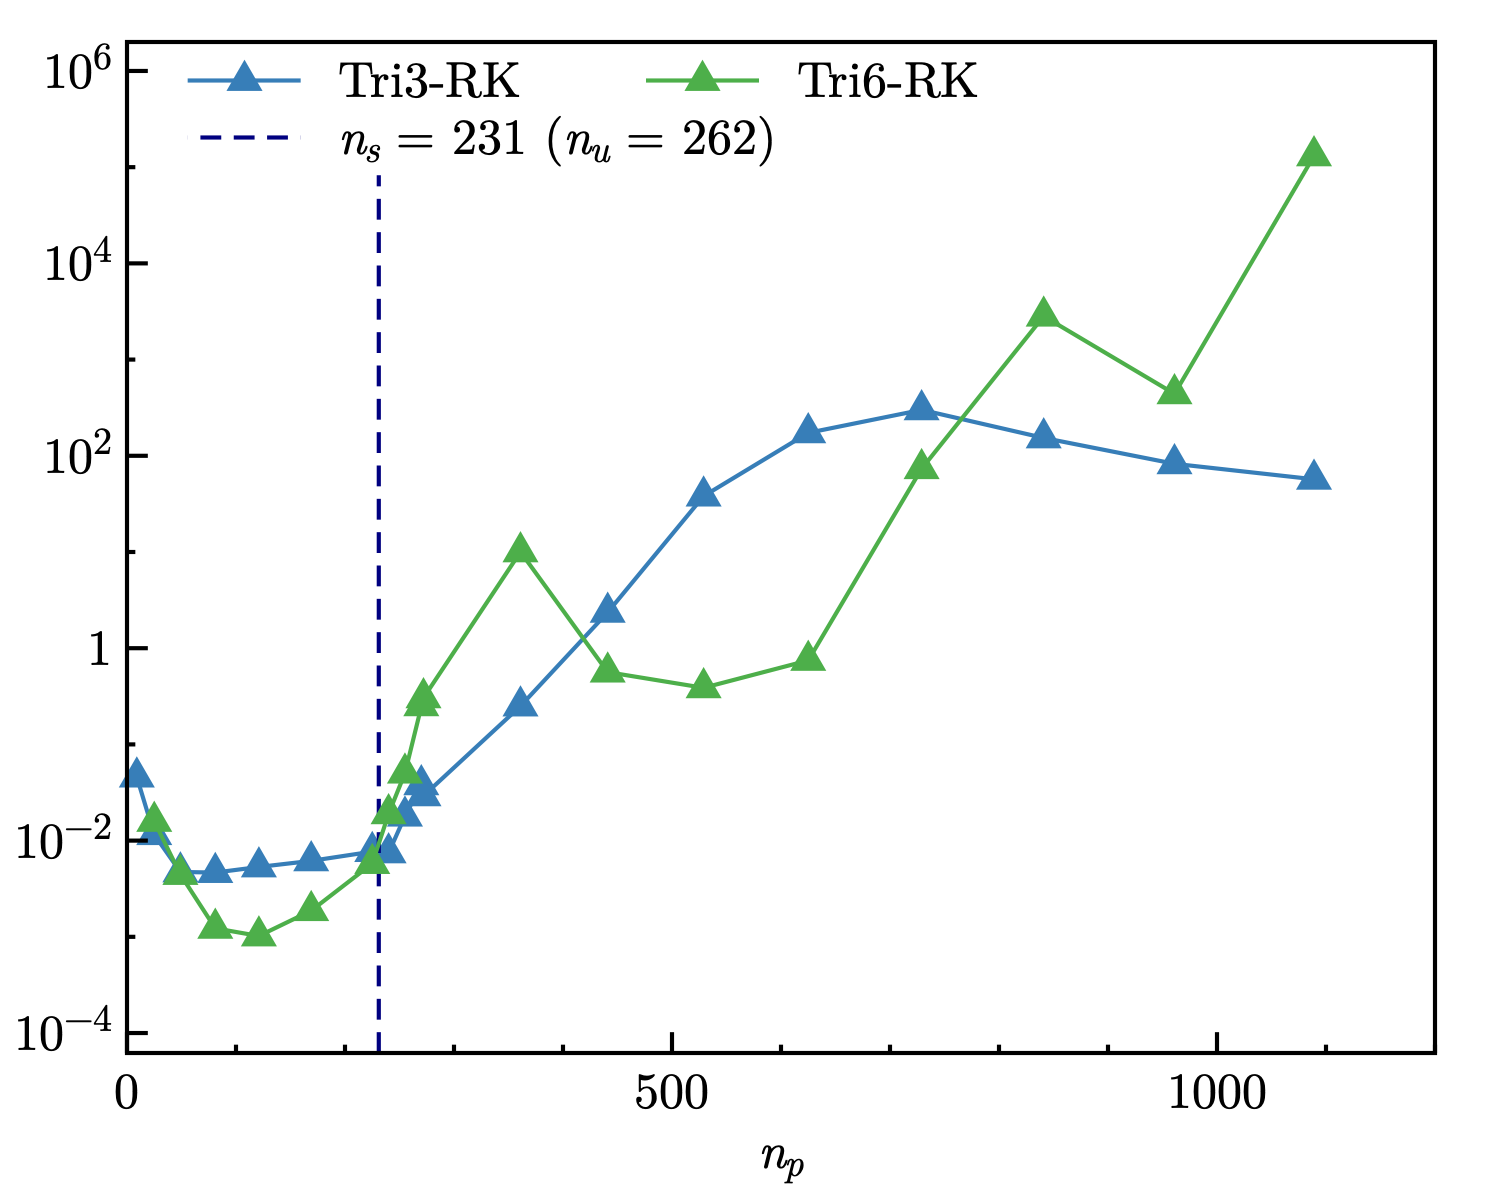
\includegraphics[width=0.48\textwidth]{png/plate_L2_p_8.png}} \\
\raisebox{-0.7\height}{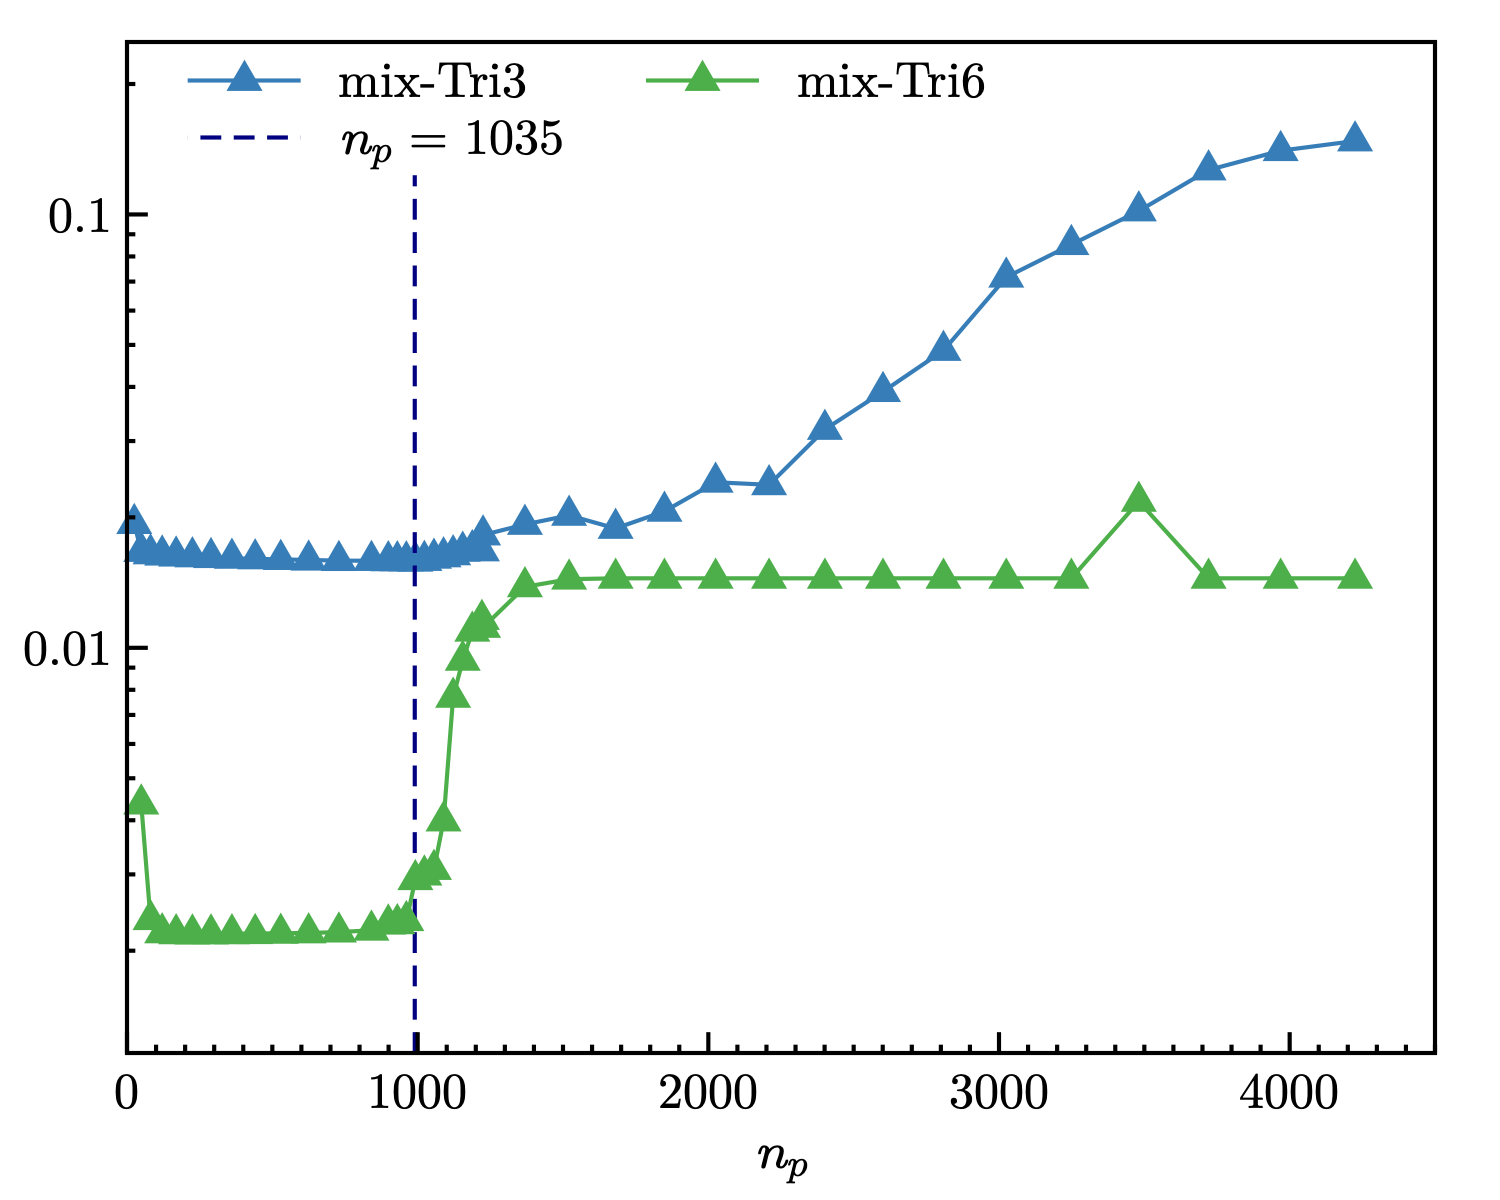
\includegraphics[width=0.48\textwidth]{png/plate_Hdev_16.png}}
& \raisebox{-0.7\height}{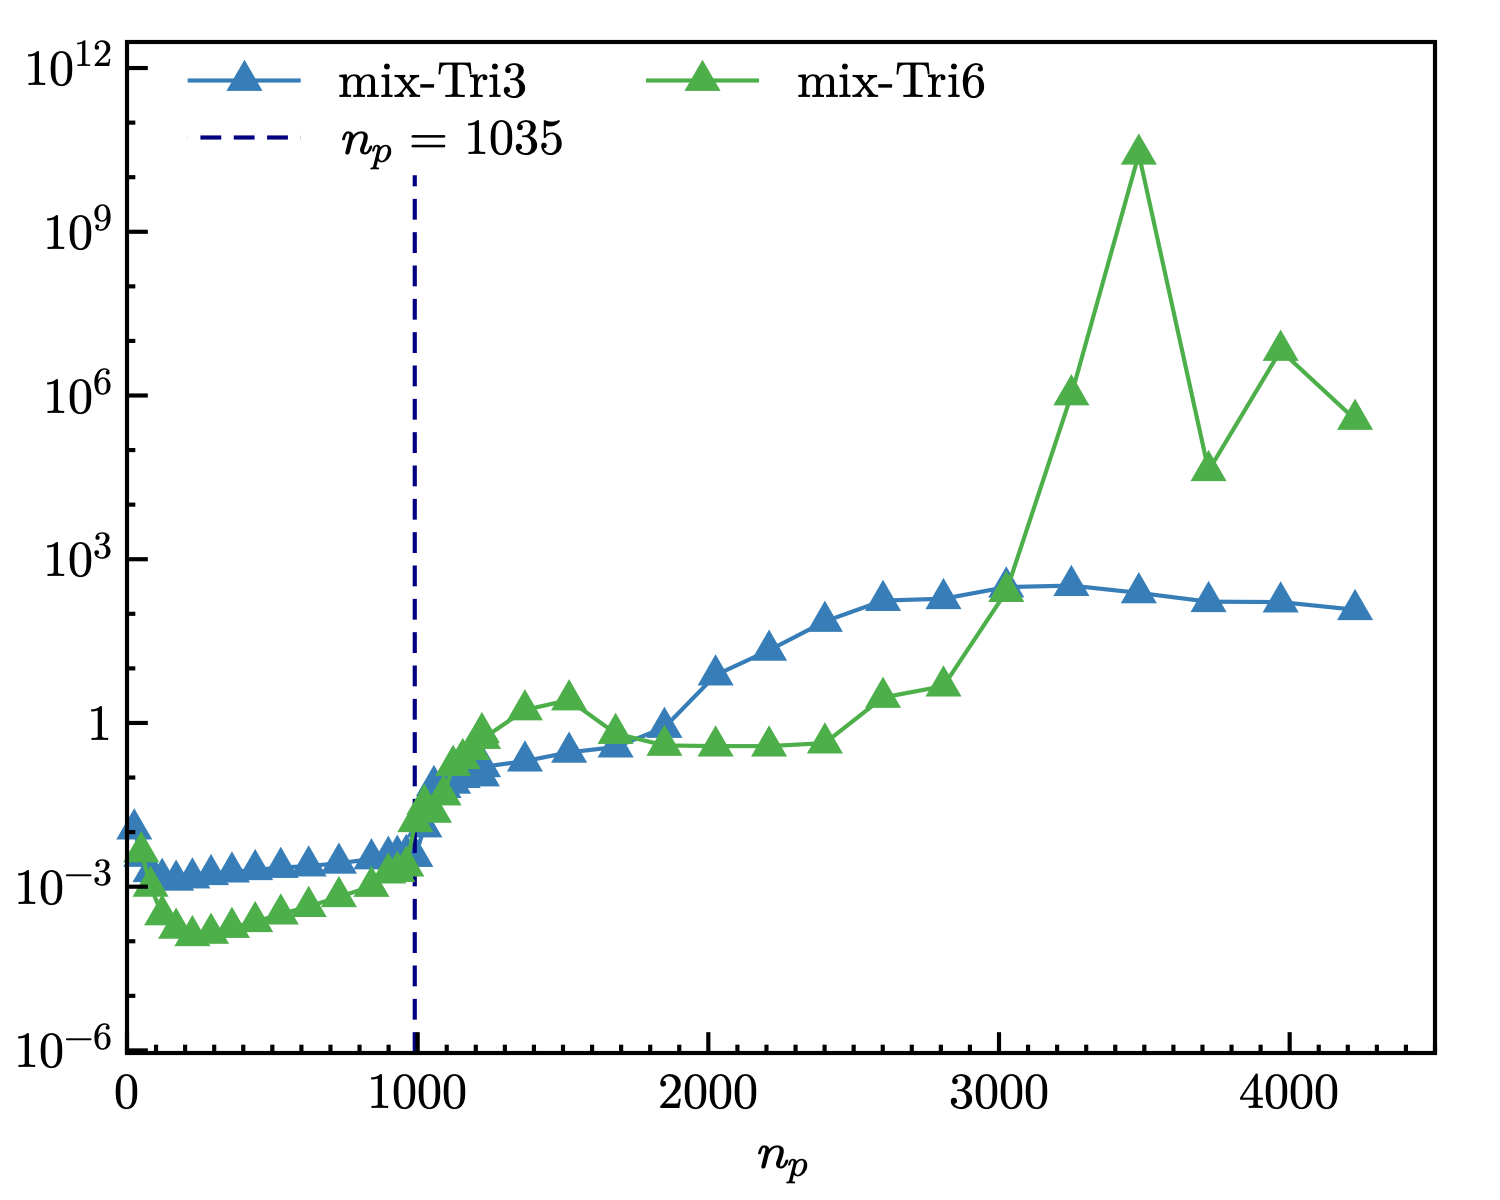
\includegraphics[width=0.48\textwidth]{png/plate_L2_p_16.png}} \\
\raisebox{-0.7\height}{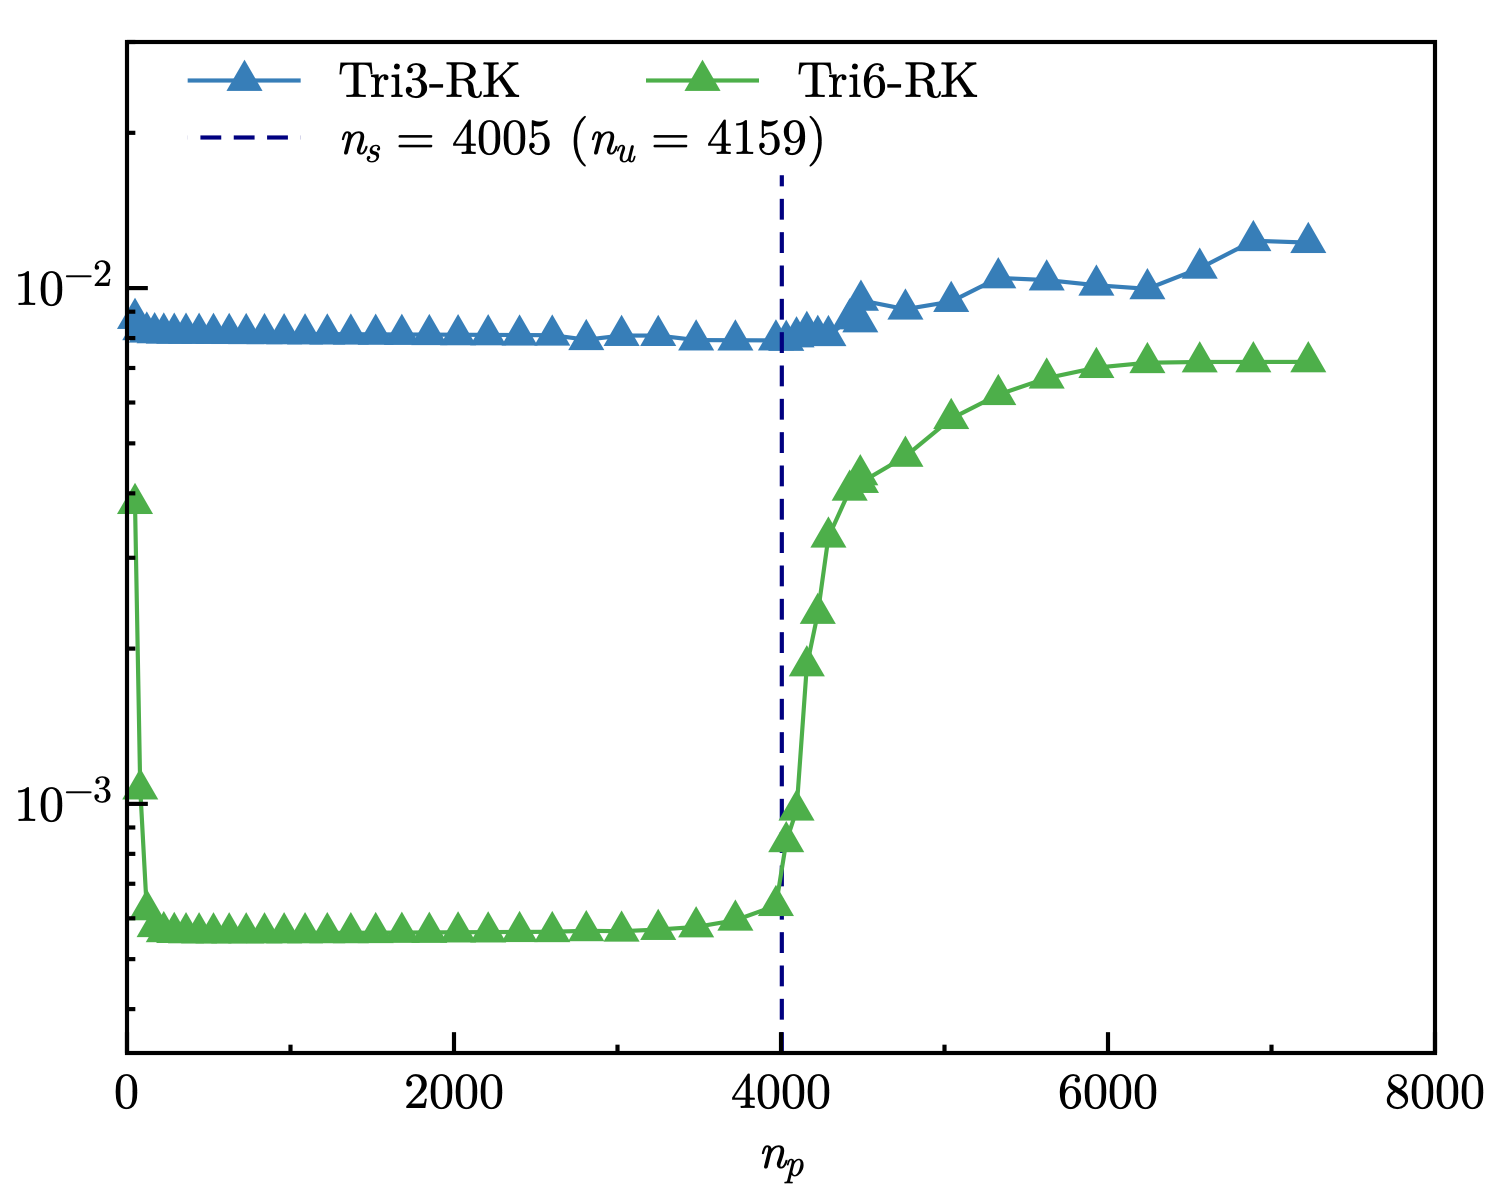
\includegraphics[width=0.48\textwidth]{png/plate_Hdev_32.png}}
& \raisebox{-0.7\height}{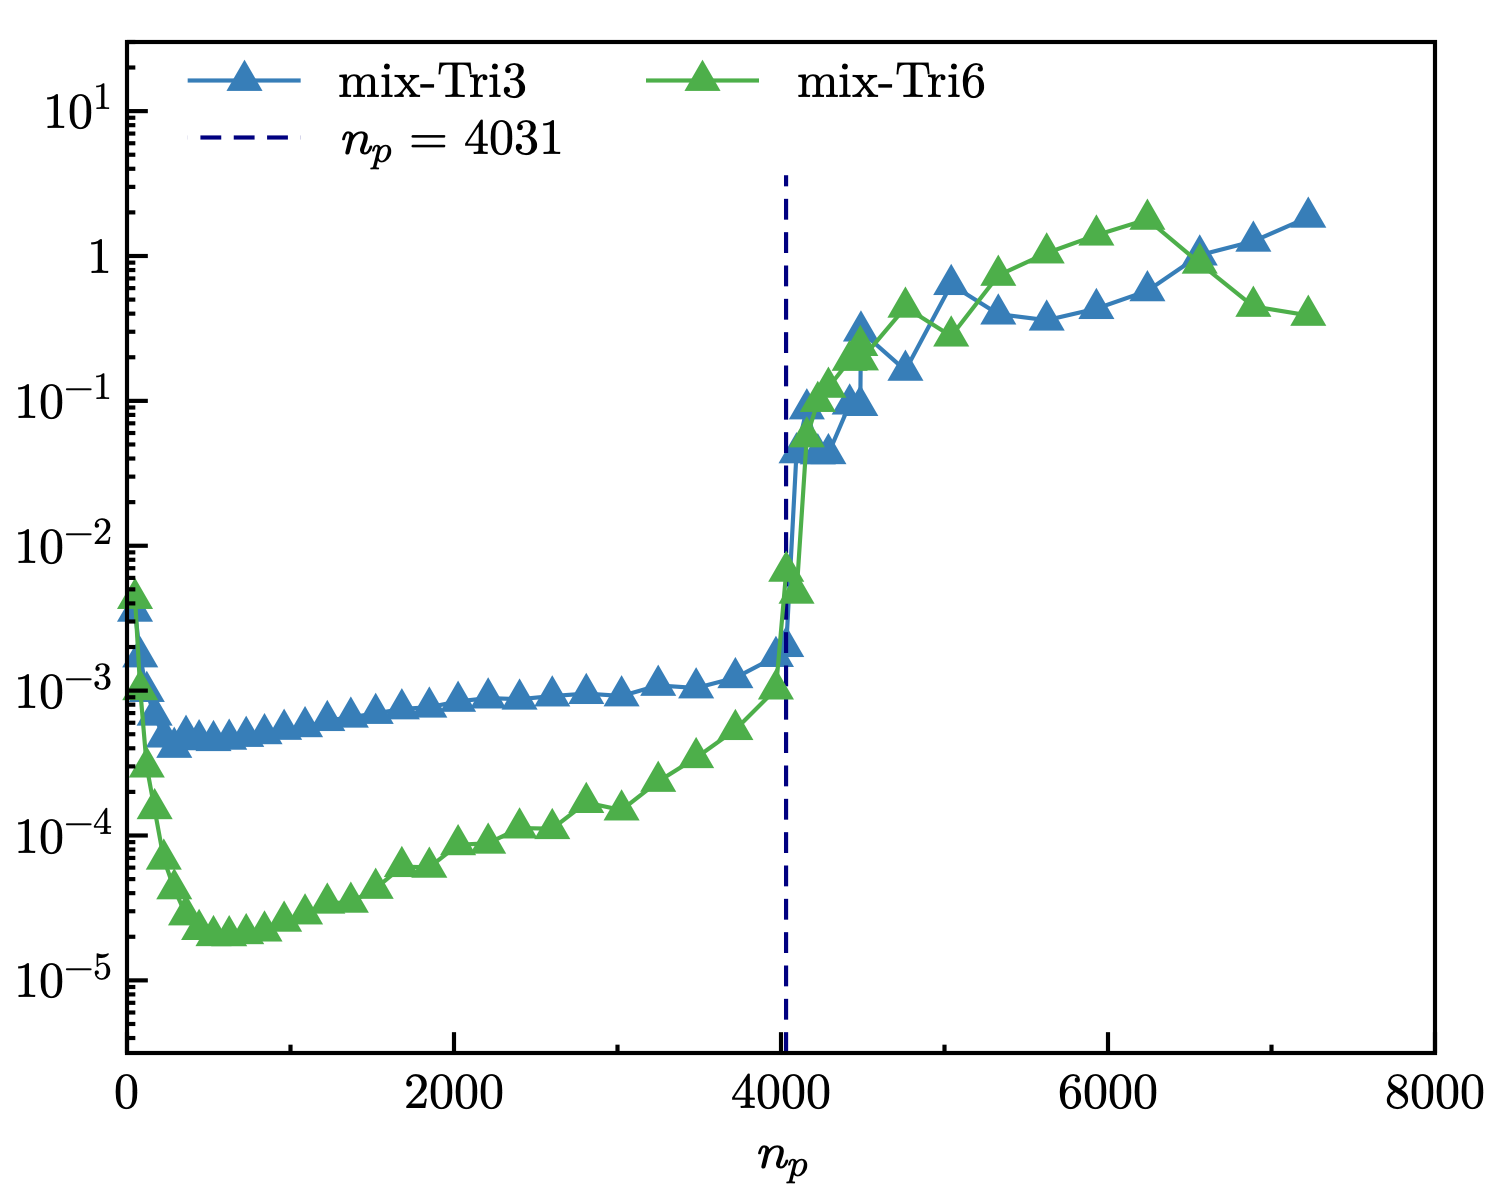
\includegraphics[width=0.48\textwidth]{png/plate_L2_p_32.png}} \\
\end{tabular}
\caption{Strain and pressure errors vs. $n_p$ for plate with hole problem}\label{fg:plate_with_hole_ns}
\end{figure}

\begin{figure}[H]
\centering
\begin{subcaptiongroup}
\centering
\parbox[b]{0.49\textwidth}{
    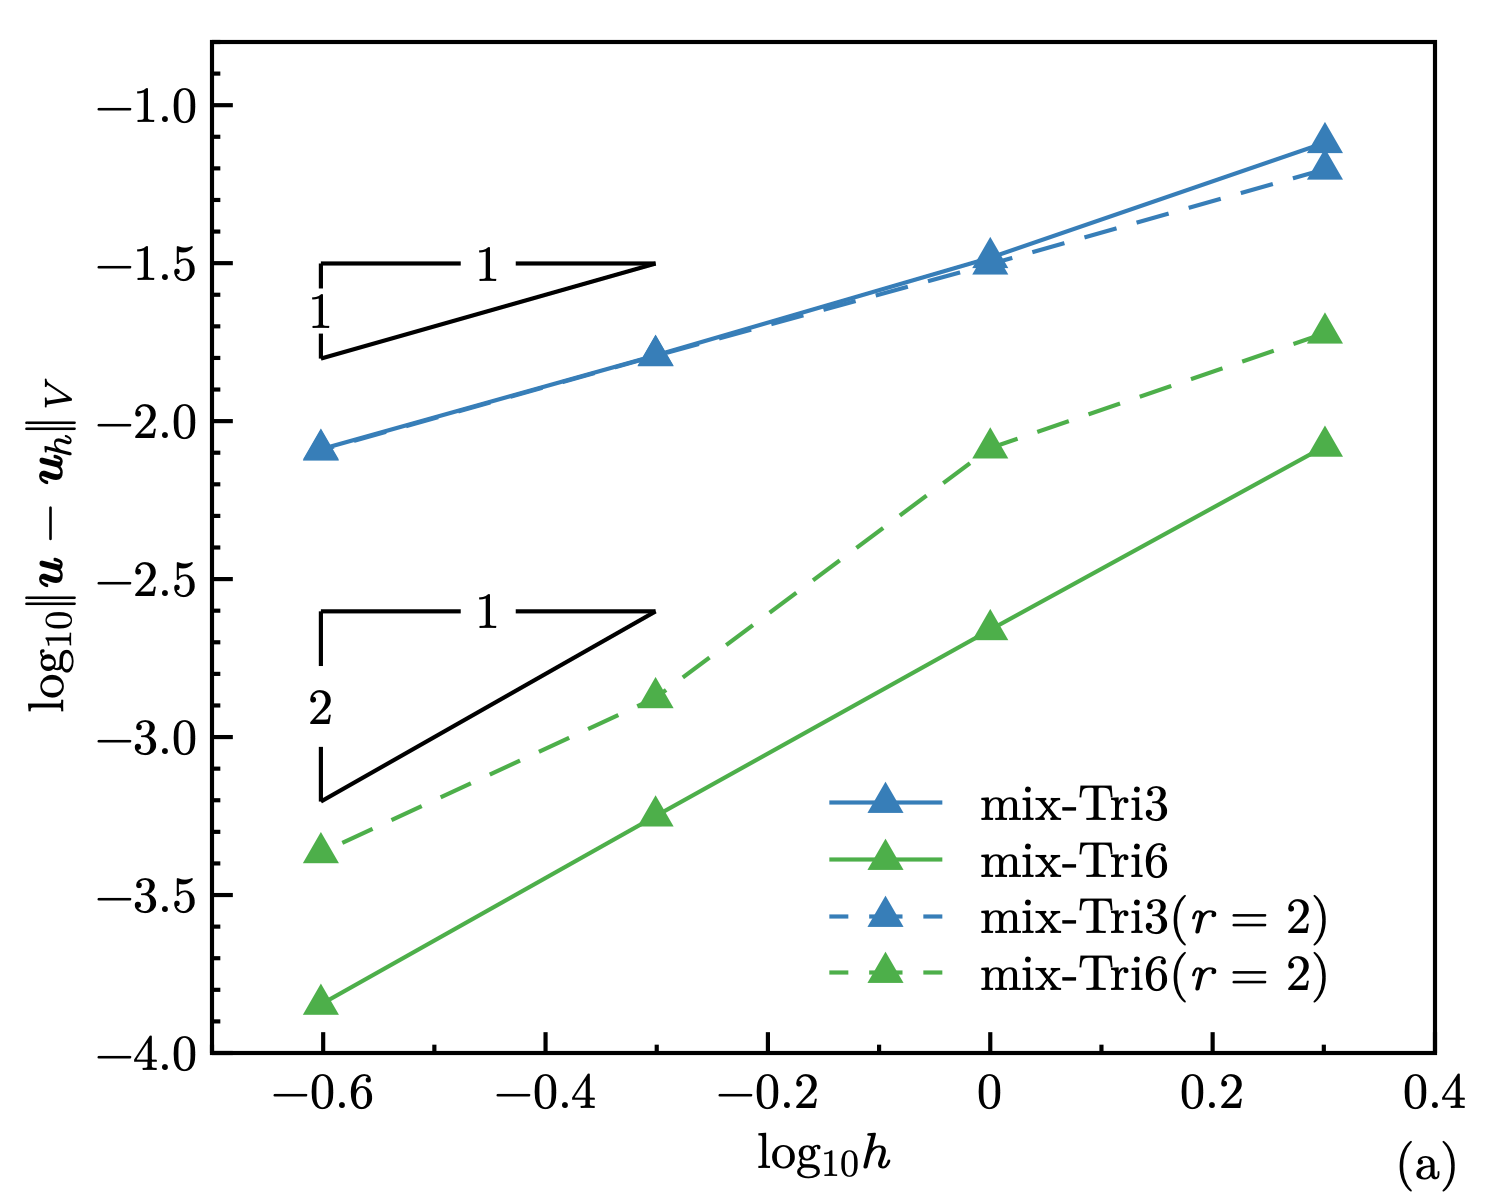
\includegraphics[width=0.49\textwidth]{png/plate_with_hole_Hdev.png}
    \caption{Strain error}\label{fg:plate_with_hole_convergence_strain}
}
\parbox[b]{0.49\textwidth}{
    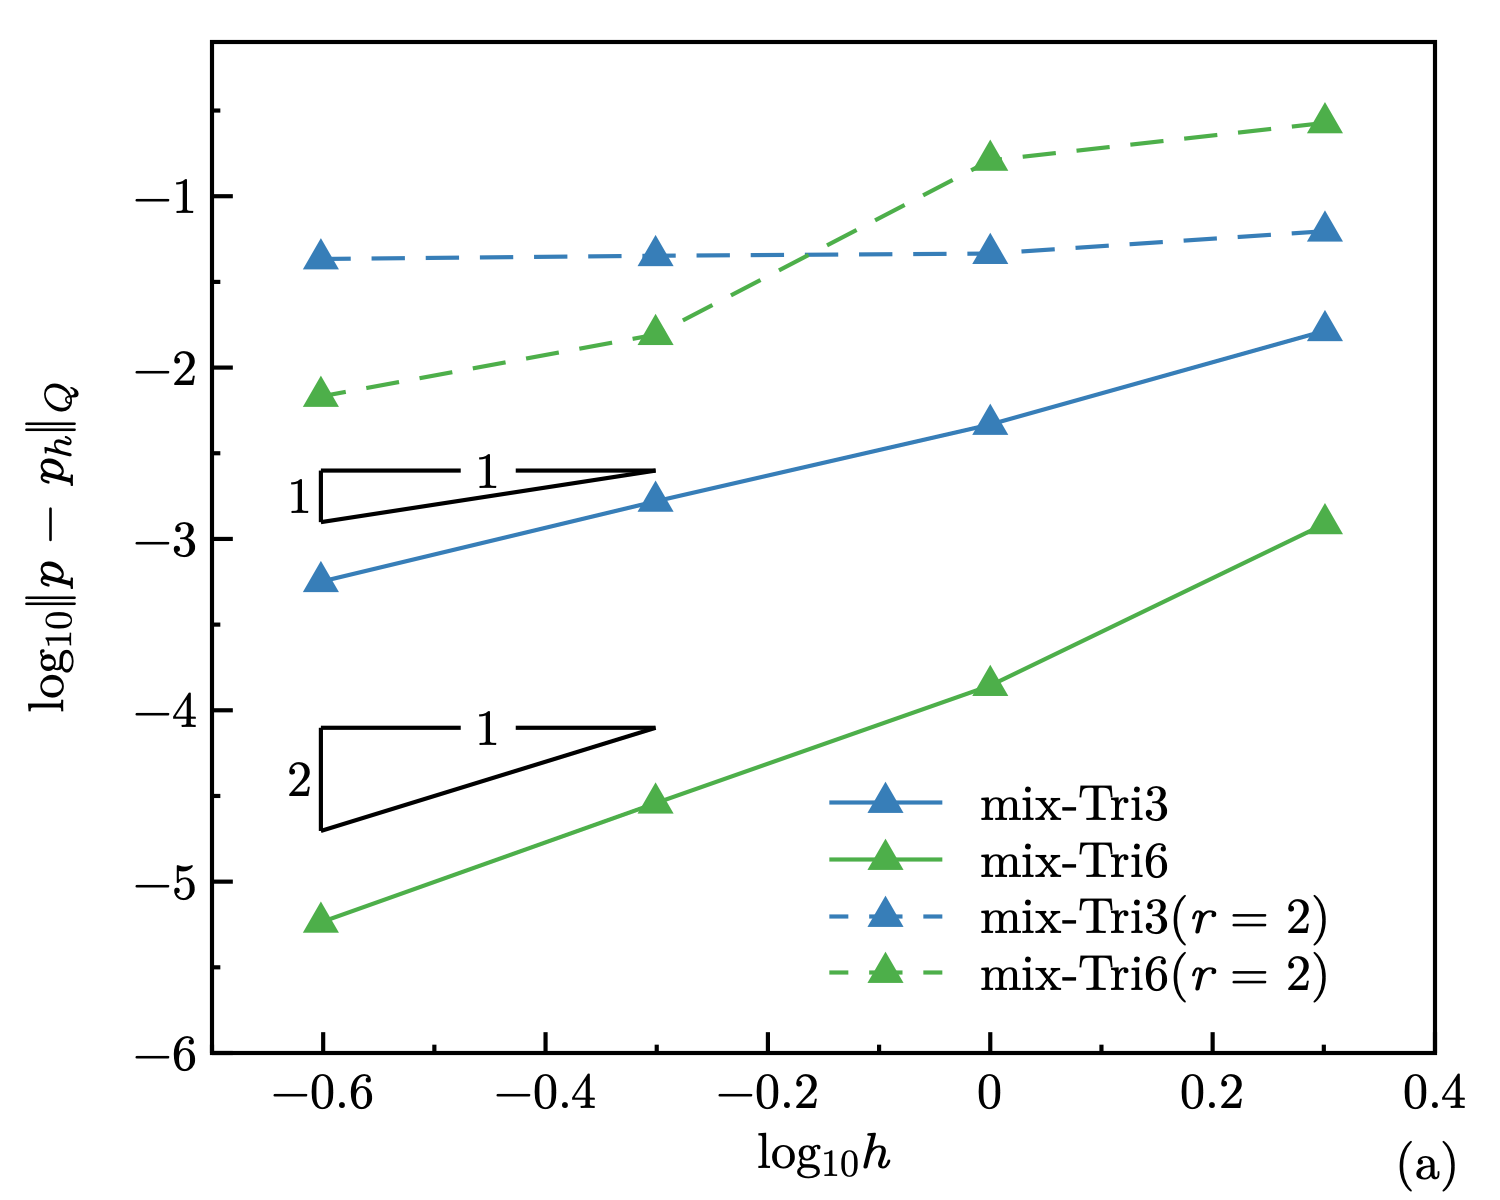
\includegraphics[width=0.49\textwidth]{png/plate_with_hole_L2_p.png}
    \caption{Pressure error}\label{fg:plate_with_hole_convergence_pressure}
}
\end{subcaptiongroup}
\caption{Error convergence study for plate with a hole problem}\label{fg:plate_with_hole_convergence}
\end{figure}

